%!TEX root = ../thesis.tex

\subsection{bang-bang制御}

\begin{figure}[H]
  \centering
 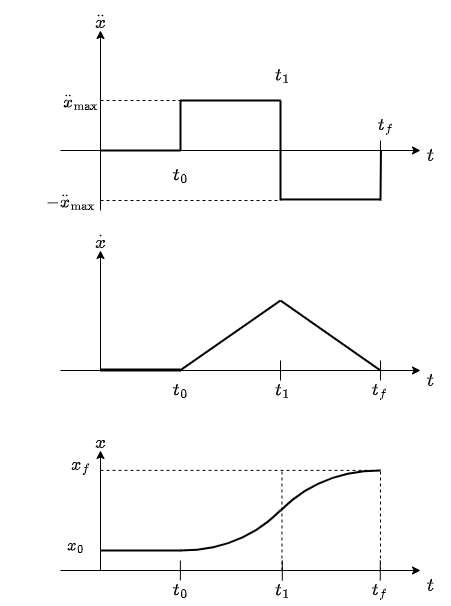
\includegraphics[keepaspectratio, scale=0.8]
      {images/png/bangbang.drawio.png}
 \caption{bang-bang control}
 \label{Fig:bangbang}
\end{figure}

速度に連続性をもたせた制御方式にbang-bang制御があり,最短時間軌道を達成できる.
最短時間軌道は,最速で目標地点に到達する際に有用な方法である.
bang-bang制御ではFig.\ref{Fig:bangbang}の加速度のグラフからわかるように,
最大加速と最小加速の2つの加速度をかけているため,最短時間で目標地点に到達することができる.
これは出発時にアクセルを全開にして,一気にブレーキをかけて,止まるというイメージである.

軌道生成及び制御を行うには初期値,目標値が必要である.今回は,位置xを変数とするため,初期値である初期位置を$x_0$,
目標値である目標位置を$x_f$,また,初速度$\dot{x}_0=0$,目標地点での速度$\dot{x}_f=0$とする.また,bang-bang制御は最大加速度$\ddot{a}_{max}$を必要とする.
このbang-bang制御を式で表すと以下のようになる.

\begin{equation} 
     \ddot{x} =
     \begin{cases}
          a & ( t_0 < t \leqq t_1 )\\
          -a & ( t_1 < t \leqq t_f )
     \end{cases}
\end{equation}

\begin{equation} 
     \dot{x} =
     \begin{cases}
          \dot{x}_0 + a(t -t_0) & ( t_0 < t \leqq t_1 )\\
          \dot{x}_1 + a(t - t_1) & ( t_1 < t \leqq t_f ) 
     \end{cases}
\end{equation}

\begin{equation}
     \text{ where $\dot{x}_1 = \dot{x}_0 + a(t_1 - t_0), \dot{x}_0 = 0$}\nonumber
\end{equation}

\begin{equation} 
     x =
     \begin{cases}
          x_0 + \frac{1}{2}a(t -t_0)^2 & ( t_0 < t \leqq t_1 )\\
          x_1 + \dot{x}_1(t-t_1) - \frac{1}{2}a(t - t_1)^2 & ( t_1 < t \leqq t_f )
     \end{cases}
\end{equation}

\begin{equation}
     \text{ where $x_1 = x_0 + \frac{1}{2}a\bigg\{\frac{(t_1 - t_0)}{2}\bigg\}^2$}\nonumber
\end{equation}

拘束条件を導出する.以上の3つの式を一般性を失わずに$t_0=0$とすると以下のようになる.

\begin{equation} 
     \ddot{x} =
     \begin{cases}
          a & ( t_0 < t \leqq t_1 )\\
          -a & ( t_1 < t \leqq t_f )
     \end{cases}
\end{equation}

\begin{equation}
     \text{ where $t_1 = \frac{t_f}{2}$}\nonumber
\end{equation}

\begin{equation} 
     \dot{x} =
     \begin{cases}
          at & ( t_0 < t \leqq t_1 )\\
          \dot{x}_1 - a(t - \frac{t_f}{2}) & ( t_1 < t \leqq t_f ) 
     \end{cases}
\end{equation}

\begin{equation} 
     \text{ where $\dot{x}_1 = a\frac{t_f}{2}$}\nonumber
\end{equation}

\begin{equation} 
     x =
     \begin{cases}
          x_0 + \frac{1}{2}at^2 & ( t_0 < t \leqq t_1 )\\
          x_1 + \dot{x}_1t - \frac{1}{2}at^2 & ( t_1 < t \leqq t_f )
     \end{cases}
\end{equation}

\begin{equation} 
     \text{ where $x_1 = x_0 + \frac{1}{2}a\Big(\frac{t_f}{2}\Big)^2$}\nonumber
\end{equation}

したがって,目標位置は
\begin{equation} 
     x_f = x_1 + \dot{x}_1t_f + a\frac{(t_f)^2}{2}
\end{equation}

となり,式(3.7)に$\dot{x}_1$,$x_1$を代入すると以下のようになる.
\begin{equation} 
     x_f = x_0 + \frac{1}{2}a\Big(\frac{t_f}{2}\Big)^2 + a\frac{t_f}{2}t_f + a\frac{(t_f)^2}{2}
\end{equation}

式(3.8)の$x_f$,$x_0$,は定数であり,変数は,目標地点への到達時間$t_f$と加速度$a$である.
最終到達時間$t_f$が決まると加速度aを求めることができ,すべての経路を決めることができる.
このときの加速度$a$は最大加速度$\ddot{x}_{max}$となる.

ここで,与える条件をまとめると以下のようになる.
\begin{description}
     \item[目標]\mbox{}\\
     $x_0, x_f$
     \item[拘束]\mbox{}\\
     $\dot{x_0}=0, \dot{x_f}=0, t_0=0, t_f$
\end{description}

\newpage
\begin{figure}[H]
     \centering
    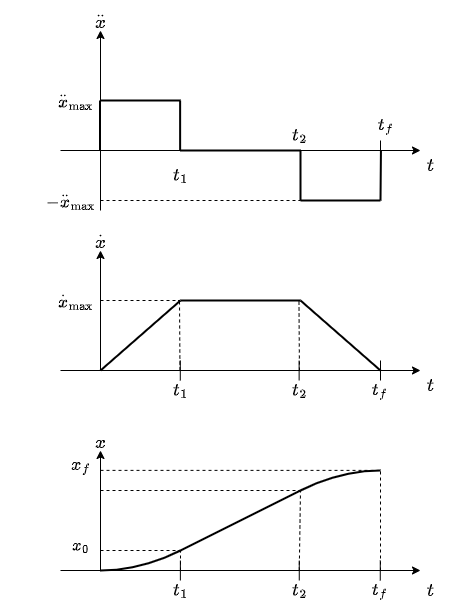
\includegraphics[keepaspectratio, scale=0.8]
         {images/png/bangbangV.drawio.png}
    \caption{bang-bang control with additional velocity constraints}
    \label{Fig:bangbangV}
\end{figure}
\newpage

bang-bang制御は加速度の変化に対応していないが,速度を変えることはできる.
拘束条件として,$\dot{x}_{max}$を追加すると,Fig.\ref{Fig:bangbangV}のようになる.
ここで$\dot{x}_{max}$は$\dot{x}_{max}=at_1$と求めることができる.
最短時間で最大速度を出すとき$\dot{x}_{max}=\ddot{x}_{max}t_1$となる.
目標地点到達時間$t_f$は$t_f=t_1+t_2$となり,$t_1$と$t_2$がわかれば,求めることができる.\\
$t_1$は$\dot{x}_{max}=\ddot{x}_{max}t_1$より\\
\begin{equation} 
     t_1=\frac{\dot{x}_{max}}{\ddot{x}_{max}}
\end{equation}
となる.\\
$t_0 < t \leqq t_1$のときの速度面積と$t_2 < t \leqq t_f$のときの速度面積は同じであるため,
$t_2$での距離は$t_0$から$t_2$までの速度が作り出す長方形の速度面積と同じになる.
したがって,$t_2$は
\begin{equation} 
     t_2=\frac{x_f-x_0}{\dot{x}_{max}}
\end{equation}
となる.\\
これにより,$\dot{x}_{max}$と$\ddot{x}_{max}$を求めることができる.

\newpage
